\section{Beyond text analysis: images, audio and video}
\label{sec:beyond}

As you may have imagined, a book about \textit{computational analysis of communication} would be incomplete without a chapter dedicated to conduct analysis over other unstructured data formats different from text. In fact, if you think of the possible contents derived from social, cultural and political dynamics in the current digital landscape, you will realize that written contents are only a limited (though potential) slide of the bigger cake. Humans produce much more oral contents than text messages, and are more agile in deciphering sounds and visual contents. Digitalization of social and political life, as well as the explosion of self-generated digital contents in the web and social media, have provoked an unprecedented amount of multimedia contents that deserve to be include in many types of research.

Just imagine a collection of digital recorded radio stations, or the enormous amount of pictures produced everyday in Instagram, or even the millions of videos of social interest uploaded in Youtube. These are definitely goldmines for social researchers who traditionally used manual techniques to analyse just a very small portion of these multimedia contents. However, it is also true that computational techniques to analyze audio, images or video are still little developed in social sciences given the difficulty of application for non-computational practitioners and the novelty of the discoveries in fields such as computer vision. 

This chapter gives a brief overview over different formats of multimedia files. We explain how to generate useful inputs into our pipeline to perform computational analysis.

You are already probably familiar with digital formats of images (.jpg, .bmp, .gif, etc.), audio (.mp3, .wav, .wma, flac, etc.) or video (.avi, .mov, .wmv, .flv, etc.), which is the very first step to use these contents as input. However, similarly to the case of texts you will need to do some preprocessing to put these formats into shape and get a proper mathematical representation of the contents. 

In the case of audio, there might be many useful computational approaches to do research over these contents: from voice recognition, audio sentiment analysis or sound classification, to automatic generation of music. Recent advances in the field of artificial intelligence have created a prosperous and diversified field with multiple academic and commercial applications. Nevertheless, computational social scientists can obtain great insights just by using specific applications such as speech-to-text transformation and then apply text analytics (already explained in this book) to the results. As you will see in \refsec{apivisions}, there are some useful libraries in R and Python to use pre-trained models to transcribe voice in different languages. 

Even when this approach is quite limited (just a small portion of the audio analytics world) and constrained (we will not address how to create the models), it will show how a specific, simple and powerful application of the automatic analysis of audio inputs can help answering many social questions (i.e. what are the topics of a natural conversation, what are the sentiments expressed in the scripts of radio news pieces, or which actors are named in oral speeches of any political party). In fact, automate analysis of audio can enable new research questions different from those typically applied to text analysis. This is the case of the research by Knox \& Lucas (FORTHCOMING), who used a computational approach over audio data from the Supreme Court Oral Arguments (407 arguments and 153 hours of audio, comprising over 66,000 justice utterances and 44 million moments) to demonstrate that some crucial information such as the scepticism of legal arguments was transmitted by vocal delivery (i.e. speech tone), something indecipherable to text analysis. Or we could also mention the work by \cite{dietrich2019pitch} who computationally analyzed the vocal pitch of more than 70,000 Congressional floor audio speeches and found that female members of the Congress spoke with greater \textit{emotional intensity} when talking about women.

On the other hand, applying computational methods to video inputs is probably the most challenging task in spite of the recent and promising advances in computer vision. For the shake of space, we will not cover specific video analytics in this chapter, but it is important to let you know that most of the computational analysis of video is based on the inspection of image and audio contents. With this standard approach you need to specify which key frames you are going to extract from the video (for example take an still image every 1,000 frames) and then apply computer vision techniques (such as object detection) to those independent images. Check for example the version 3 of the object detection architecture \textit{You Only Look Once Take} (YOLOv3)\footnote{https://pjreddie.com/darknet/yolo/} created by \citet{yolov3}, which uses a pre-trained Convolutional Neural Network (CNN) (see section \refsec{cnn}) to locate objects within the video (figure~\ref{fig:yolo}). To answer many social science questions you might complement this frame-to-frame image analysis with an analysis of audio features. In any case, this approach will not cover some interesting aspects of the video such as the camera frame shots and movements, or the editing techniques, which certainly give more content information.

\begin{figure}
\centering
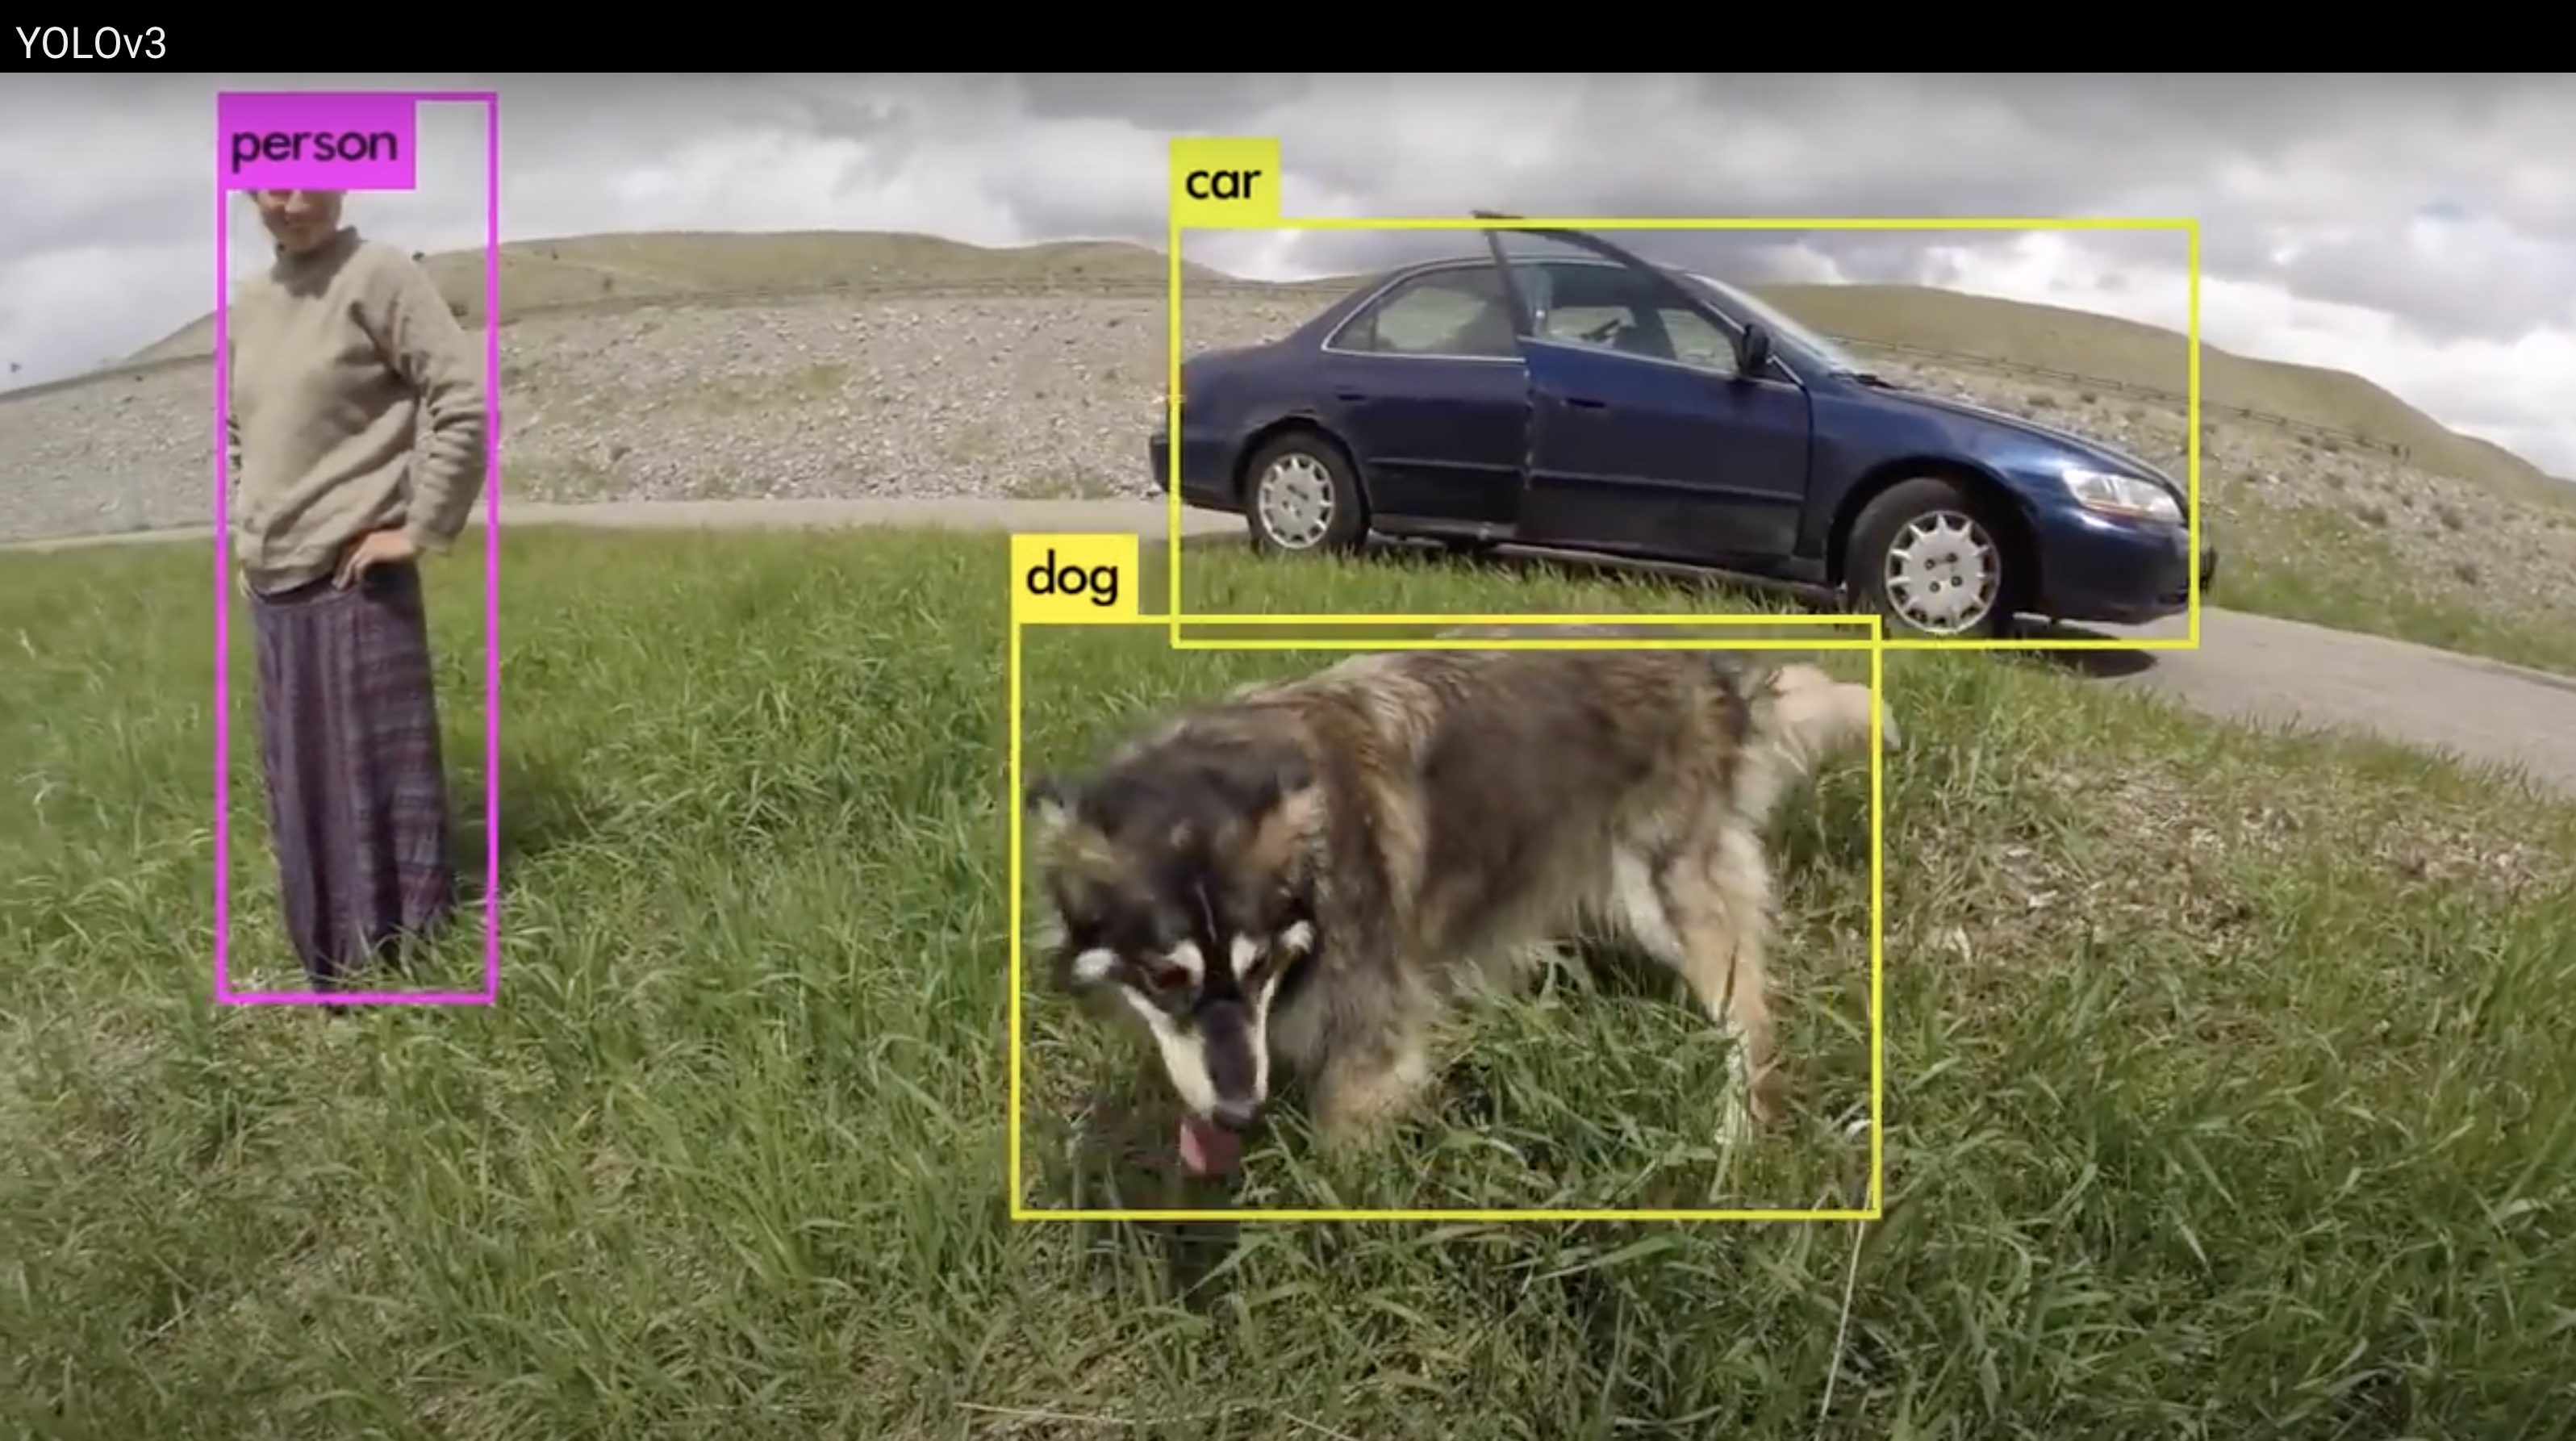
\includegraphics[width=0.9\linewidth]{figures/ch15_yolo.png}
\caption{A screen shot of a real-time video analyzed by YOLOv3 in its webpage https://pjreddie.com/darknet/yolo/}
\label{fig:yolo}
\end{figure}
